\documentclass{standalone}
\usepackage{tikz}
\usetikzlibrary{decorations.pathreplacing}

\begin{document}
  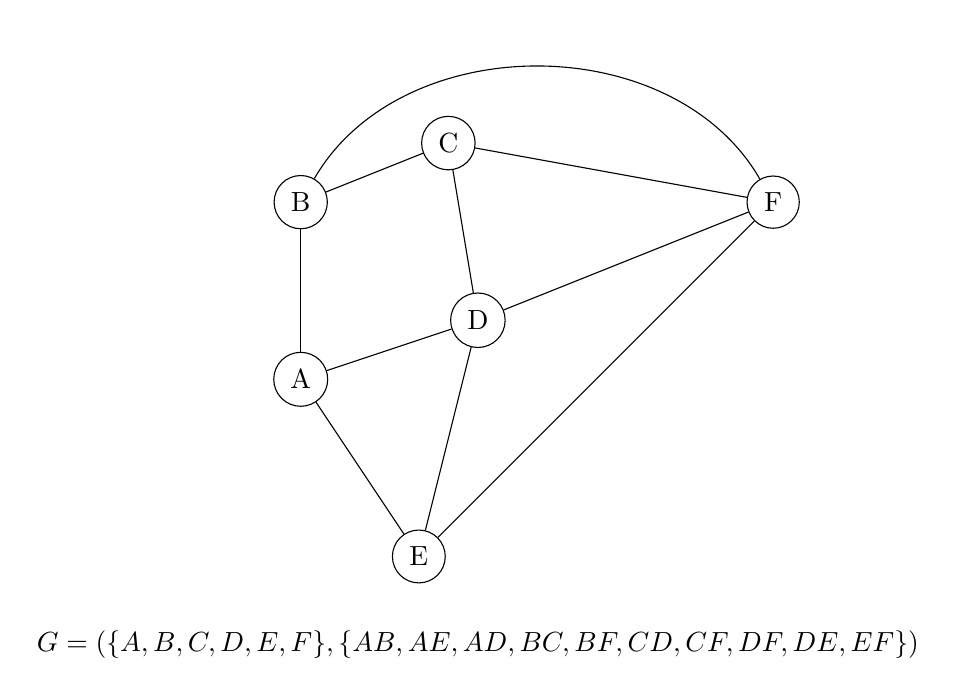
\begin{tikzpicture}[scale=0.75]
    \node[shape=circle,draw=black] (A) at (0,0) {A};
    \node[shape=circle,draw=black] (B) at (0,3) {B};
    \node[shape=circle,draw=black] (C) at (2.5,4) {C};
    \node[shape=circle,draw=black] (D) at (3,1) {D};
    \node[shape=circle,draw=black] (E) at (2,-3) {E};
    \node[shape=circle,draw=black] (F) at (8,3) {F} ;
    \node (L) at (3,-4.5) {\(G=(\{A,B,C,D,E,F\}, \{AB,AE,AD,BC,BF,CD,CF,DF,DE,EF\})\)};

    \path (A) edge (B);
    \path (B) edge (C);
    \path (B) edge [bend left=60] (F);
    \path (A) edge (D);
    \path (D) edge (C);
    \path (A) edge (E);
    \path (D) edge (E);
    \path (D) edge (F);
    \path (C) edge (F);
    \path (E) edge (F);
  \end{tikzpicture}
\end{document}
